\subsection{Equações de movimento}
As equações de movimento descrevem a trajetória de um elétron se movendo próximo da órbita ideal, com uma energia próxima, mas não necessariamente igual, à energia nominal $E_0$. O desvio de energia é definido como
\begin{align}
	\epsilon = E-E_0
\end{align}
onde $E$ é a energia do elétron.

Para manter a aproximação linear, são considerados apenas pequenas quantidades de $x$, $z$ e $\epsilon$. Melhor do que tomar o tempo como variável independente, é mais conveniente adotar a coordenada longitudinal $s$. Assim, derivadas com relação a $s$ serão indicadas daqui pra frente pela notação $(')$. Por exemplo, $x'=\frac{dx}{ds}$.

Começando a análise pelo movimento radial. Considere um elétron em $x$ movendo-se com inclinação $x'$ (Figura \ref{fig:fig9}). A inclinação é o ângulo entre a direção do movimento do elétron e a tangente à órbita ideal. $x'$ é o ângulo entre a trajetória e a tangente à órbita ideal. Suponha um ângulo $\theta_0$ entre a tangente e uma direção de referência arbitrária e um ângulo $\theta$ entre a trajetória e a mesma direção de referência. Logo, $x' = \theta-\theta_0$ e
\begin{align}
	x'' = \frac{d(\theta-\theta_0)}{ds}\label{eq:2.12}
\end{align}

\begin{figure}[!htb]
	\centering
	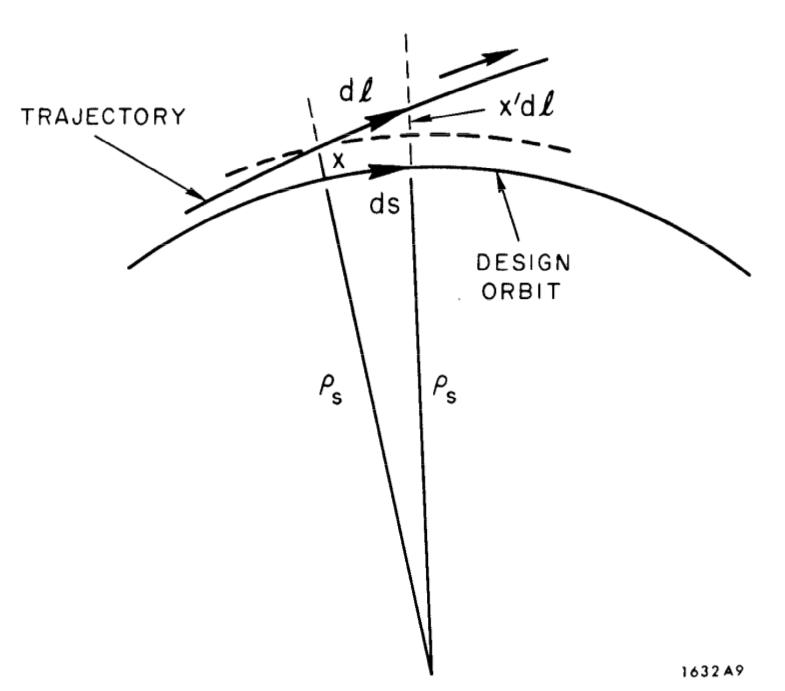
\includegraphics[width=0.6\linewidth]{./Figuras/fig9.jpeg}
	\caption{Trajetória de um elétron próxima à órbita ideal. Retirado de \cite{sands1970physics}.}
	\label{fig:fig9}
\end{figure}

A derivada de $\theta_0$ é, como já foi visto, $\frac{-1}{\varrho_s} = G(s)$ ($\varrho_s = \varrho(s)$). Mas o que é $\frac{d\theta}{ds}$? O rario de curvatura da trajetória é
\begin{align}
	\varrho = \frac{E}{ecB}
\end{align}
e, em um elemento de caminho $d\ell$ da trajetória, a variação do ângulo é
\begin{align}
	d\theta = -\frac{d\ell}{\varrho} = -\frac{ecB}{E}d\ell\label{eq:2.14}
\end{align}

Note que, enquanto o ângulo $x'$ é pequeno -- e pode-se sempre assumir isto desde que apenas termos de primeira ordem sejam considerados, que é o caso -- um elemento de caminho $d\ell$ da trajetória em $x$ é relacionado com a correspondente variação em $s$ por
\begin{align}
	d\ell = \frac{\varrho_s - x}{\varrho_s} ds = \left(1+\frac{x}{\varrho_s}\right)ds = (1+G(s))ds\label{eq:2.15}
\end{align}

Agora, $B$ pode ser descrito por
\begin{align}
	B = B_0 + \frac{\partial B}{\partial x}x = \frac{E_0}{ec}(G+K_1x)\label{eq:2.16}
\end{align}

Substituindo as equações \eqref{eq:2.15} e \eqref{eq:2.16} na equação \eqref{eq:2.14} juntamente com $E_0+\epsilon$ para $E$ -- e mantendo apenas termos de primeira ordem -- tem-se que
\begin{align}
	d\theta = \left\{-G-(G^2+K_1)x + G\frac{\epsilon}{E_0}\right\}ds
\end{align}
e, portanto, 
\begin{align}
	x'' = -(G^ 2+K_1)x + G\frac{\epsilon}{E_0}
\end{align}

\begin{proof}
	Pela equação \eqref{eq:2.14},
	\begin{align*}
		d\theta &= -\frac{ecB}{E}d\ell\\
				&= -\frac{ecB}{E}(1+Gx)ds\\
				&= -\frac{ec}{E}\left[\frac{E_0}{ec}(G+K_1x)\right](1+Gx)ds\\
				&= -\frac{E_0}{E_0+\epsilon}(G+K_1x)(1+Gx)ds\\
				&= -\frac{E_0}{E_0+\epsilon}(G+K_1x+G^2x+K_1Gx^2)ds\\
				&= -\frac{E_0}{E_0+\epsilon}(G+(G^2+K_1)x + K_1Gx^2)ds
	\end{align*}
	
	Mantendo apenas termos de primeira ordem para continuar com a aproximação linear,
	\begin{align*}
		d\theta &= -\frac{E_0}{E_0+\epsilon}(G+(G^2+K_1)x)ds\\
				&= \frac{E_0}{E_0+\epsilon}(-G-(G^2+K_1)x)ds\\
				&= \frac{1}{1+\epsilon/E_0}(-G-(G^2+K_1)x)ds\\
	\end{align*}
	
	Como $\epsilon/E_0$ é bem pequeno, pode-se considerar que o termo $\frac{1}{1+\epsilon/E_0}$ é a soma de uma série geométrica. Logo, pode-se expandir este termo em um somatório:
	\begin{align*}
		d\theta &= \left(1 - \frac{\epsilon}{E_0} + \frac{\epsilon^2}{E_0^2}+ ...\right)(-G-(G^2+K_1)x)ds
	\end{align*}
	
	Novamente, mantendo apenas termos de primeira ordem,
	\begin{align*}
		d\theta &= \left(1 - \frac{\epsilon}{E_0}\right)(-G-(G^2+K_1)x)ds\\
				&= (-G-(G^2+K_1)x)ds + \left(G\left(\frac{\epsilon}{E_0}\right)+(G^2+K_1)x\left(\frac{\epsilon}{E_0}\right)\right)ds
	\end{align*}
	
	Aplicando novamente o argumento acima,
	\begin{align*}
		d\theta = \left\{-G-(G^2+K_1)x + G\frac{\epsilon}{E_0}\right\}ds
	\end{align*}
	
	Agora, pela equação \eqref{eq:2.12},
	\begin{align*}
		x'' &= \frac{d(\theta-\theta_0)}{ds}\\
			&= \frac{\left\{-G-(G^2+K_1)x + G\frac{\epsilon}{E_0}\right\}ds - (-G)ds}{ds}\\
			&= -(G^2+K_1)x + G\frac{\epsilon}{E_0}
	\end{align*}
\end{proof}

A equação correspondente para o movimento vertical é
\begin{align}
	z'' = K_1 z
\end{align}

\begin{proof}
	Para $z''$, pela força de Lorentz,
	\begin{align*}
		d\theta &= -\frac{d\ell}{\varrho} = + \frac{ecB}{E}d\ell\\
				&= \frac{ecB}{E}d\ell\\
				&= \frac{ecB}{E}(1+Gx)ds\\
				&= K_1 z (1+Gx)ds\\
				& = (K_1 z + GK_1xz)ds
	\end{align*}
	
	Descartando o termo de segunda ordem,
	\begin{align*}
		d\theta &= K_1 z ds\\
	\end{align*}
	
	Agora, pela equação \eqref{eq:2.12},
	\begin{align*}
		z'' &= \frac{d(\theta-\theta_0)}{ds}\\
			&= \frac{K_1 z\ ds}{ds}\\
			&= K_1 z
	\end{align*}
	lembrando que $\frac{d\theta_0}{ds} = 0$ porque não há componente vertical nesta variação.
\end{proof}

Definindo as funções focalizadoras $K_x$ e $K_z$ como
\begin{align}
	K_x(s) &= G^2(s)+K_1(s)\label{eq:2.21}\\
	K_z(s) &= - K_1(s)
\end{align}
tem-se que $x''$ e $z''$ podem ser descritos como
\begin{align}
	x'' &= -K_x(s)x + G(s)\frac{\epsilon}{E_0}\label{eq:2.19}\\
	z'' &= -K_z(s)z\label{eq:2.20}
\end{align}

O termo correspondente à $G^2$ está "faltando" de $K_z$ devido à consideração de que a órbita ideal está no plano, ou seja, não possui componente vertical. Mais especificamente, $G^2$ é um termo de força centrífuga, e um termo correspondente apareceria no movimento vertical se a órbita tivesse picos e vales. Anéis de armazenamento possuem, em geral, uma forte focalização. Neste caso, $G^2$ é bem menor que $K_1$, então $K_x$ e $K_z$ são aproximadamente iguais e possuem sinais opostos. Fisicamente, esta diferença de sinal significa que um elemento focalizador que focaliza em $x$ automaticamente desfocaliza em $z$, e vice-versa.

A equação de movimento em $z$ parece a equação de uma oscilação clássica (força proporcional ao desvio), com um coeficiente de força restauradora variável -- a função $K_z(s)$. A equação em $x$ é similar, exceto pela adição de um termo variável proporcional ao desvio de energia $\epsilon$. Nos campos guia que podem ser efetivamente utilizados, as soluções destas equações são, na verdade, oscilatórias, e descrevem oscilações laterais -- incluindo as chamadas oscilações betatron -- na trajetória do elétron. Estas oscilações são resultado das propriedades focalizadoras do campo guia, as quais caracterizam as funções de focalização $K_x$ e $K_z$.

Tanto $K_x$ quanto $K_z$ são funções periódicas ao longo do anel, logo
\begin{align}
	\begin{array}{rcl}
	\ K(s+L) & = & K(s)
	\end{array}
\end{align}

Por conveniência na construção e no design do anel, este possui uma periodicidade intrínseca. Ou seja, é composta por uma sequência de células magnéticas idênticas, cada célula sendo constituída por dipolos e quadrupolos. Então, para um anel com células de comprimento $\ell_c$,
\begin{align}
	\left\{\begin{array}{rcl}
	\ G(s+\ell_c) & = & G(s)\\
	K(s+\ell_c) & = & K_1(s)
	\end{array}\right.
\end{align}

Nota-se que, diferentemente da primeira propriedade, a periodicidade de célula é uma propriedade do design da máquina, não sendo totalmente verdadeira em campos reais devido a imperfeições na construção.

Na \autoref{fig:fig10}, a natureza das funções de focalização em uma parte do anel, abrangendo duas células. A Figura \ref{fig:fig10} (a) mostra o configuração dos dipolos e quadrupolos do anel. Os dipolos são denominados por B e tem um campo uniforme ($dB/dx = 0$). Os quadrupolos não tem campo na órbita ideal ($B_0=0$) e são denominados por F e D (F para focalizador e D para desfocalizador, ambos com relação ao movimento radial). As Figuras \ref{fig:fig10} (b) e (c) são as funções de focalização $G$, $K_x$ e $K_z$.

\begin{figure}[!htb]
	\centering
	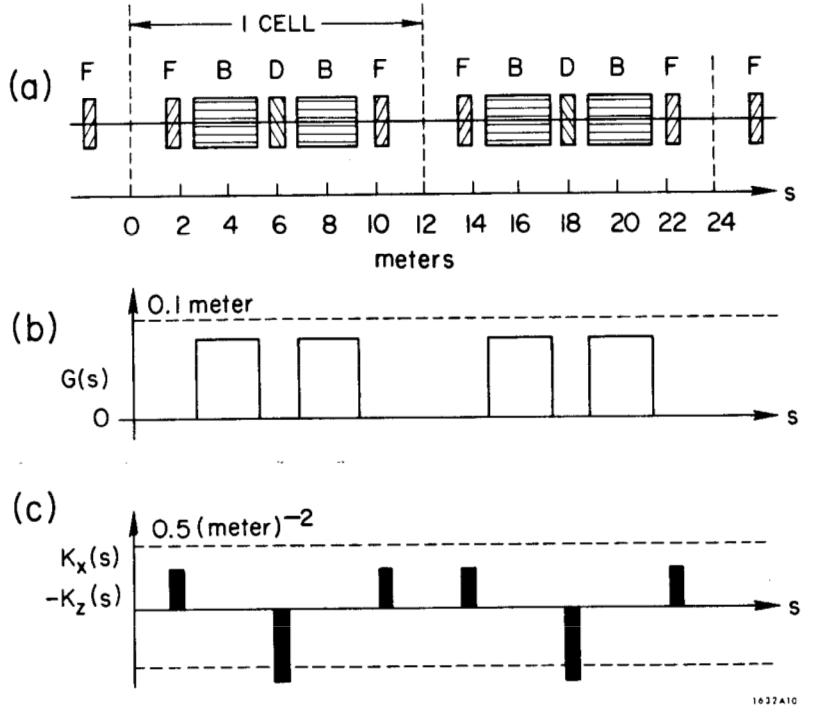
\includegraphics[width=0.7\linewidth]{./Figuras/fig10.jpeg}
	\caption{Laço magnético e funções de focalização em uma célula de um campo guia em particular. Retirado de \cite{sands1970physics}.}
	\label{fig:fig10}
\end{figure}